\section{Task Maintenance}

Managing Tasks
\newline
Tasks can be created and added to a story from within the story editor. To begin, expand the task section.

\begin{figure}[H]
\centering
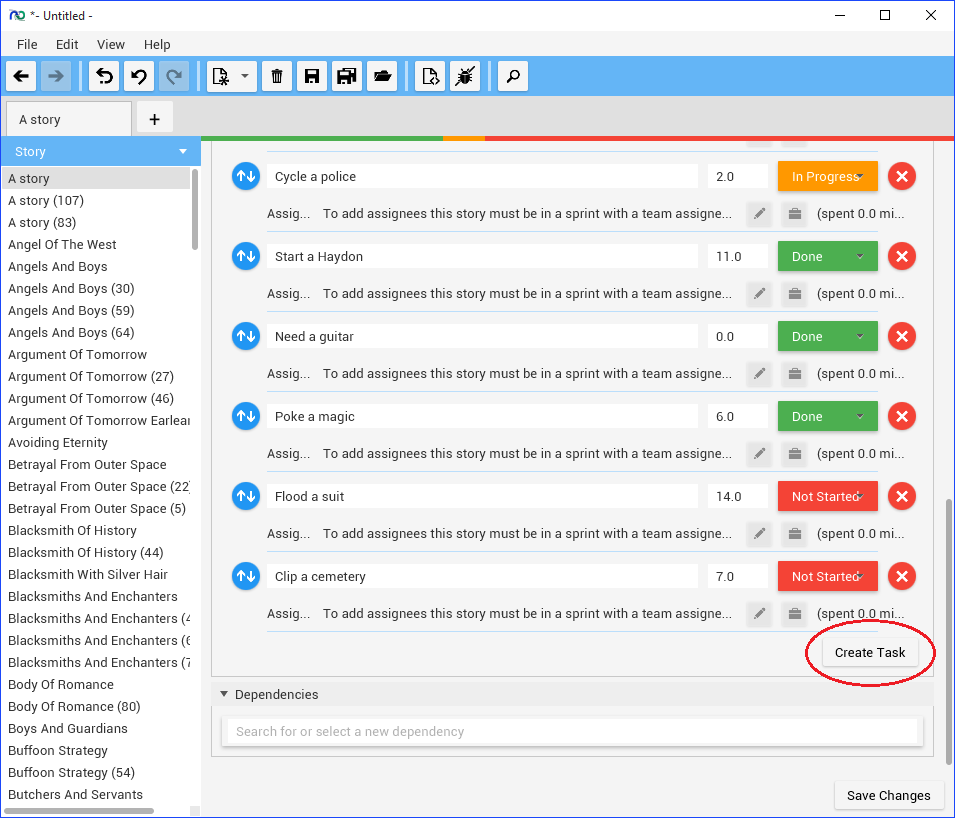
\includegraphics[width=\textwidth]{images/screenshots/task_1.png}
\caption{Create a new task}
\label{fig:new_project}
\end{figure}

Click on the "Create Task" button, circled in red. It will add a new blank task for you to fill the details in for.

\begin{figure}[H]
\centering
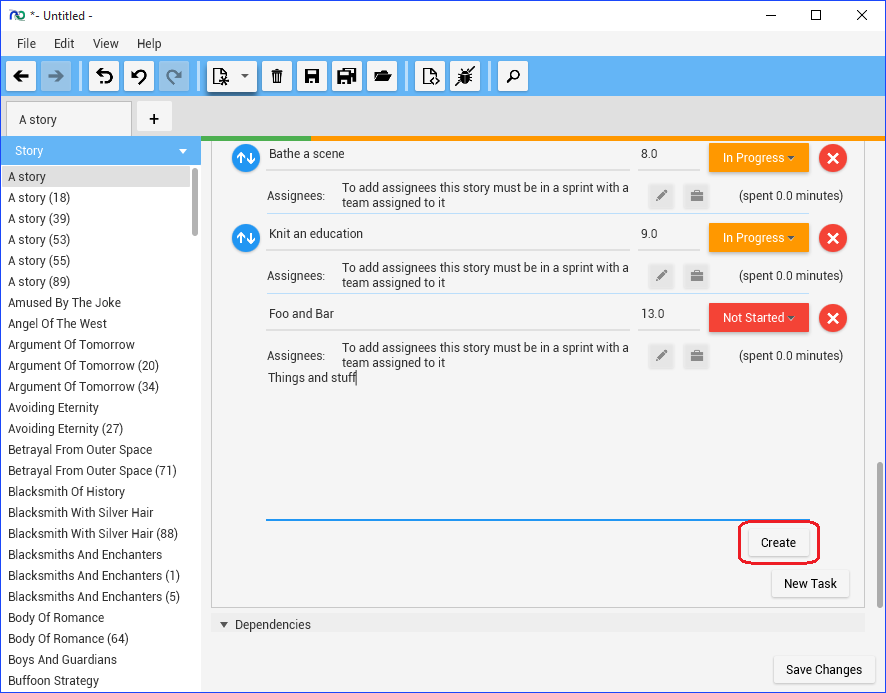
\includegraphics[width=\textwidth]{images/screenshots/task_2.png}
\caption{Save the newly created task}
\label{fig:new_project}
\end{figure}

Once the name and estimate fields have valid values entered, you will be able to click on the "Create" button and save the task to that story. Now, it will always be there when you come back to that story.

\newline

Note:
\newline
You cannot make two tasks with the same name.